% example.tex
\documentclass[dvisvgm]{standalone}

\usepackage{amsmath}
\usepackage[usenames,dvipsnames]{xcolor}
\usepackage{tikz}
\usetikzlibrary {arrows.meta,
                 calc,
                 positioning,
                 shapes.geometric}

 \tikzset{
        base/.style={draw, align=center, minimum height=4ex},
        proc/.style={base, rectangle, text width=8em},
        io/.style={trapezium, trapezium left angle=70, trapezium right
                   angle=110, draw, text width=8em, %minimum width=2cm, 
                   %minimum height=1cm
                   },
        test/.style={base, diamond, aspect=2,
                     %text width=5em
                     },
        term/.style={proc, rounded corners},
        myarrow/.style={-Stealth, line width=0.25mm},
 }

\begin{document}
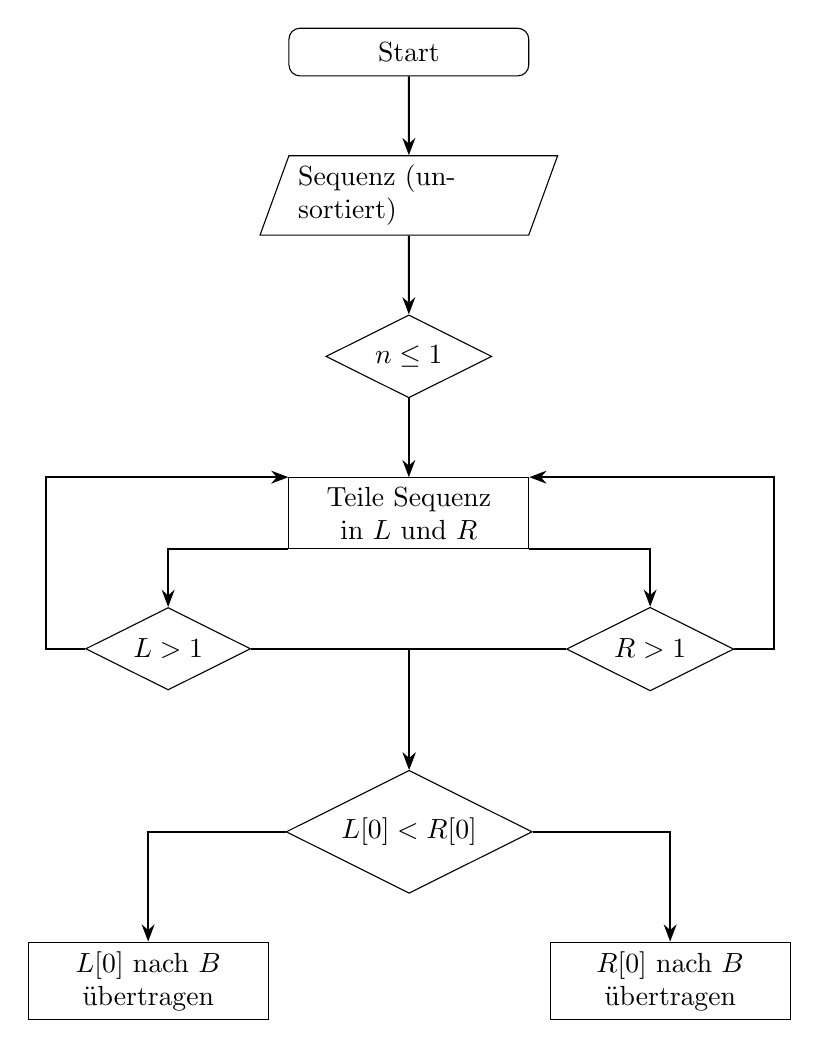
\begin{tikzpicture}
    \node[draw, term] (a) {Start};
    \node[draw, io, below= of a] (b) {Sequenz (unsortiert)};
    \node[draw, test, below= of b] (c) {$n\leq 1$};
    \node[draw, proc, below= of c] (d) {Teile Sequenz in $L$ und $R$};
    \node[draw, test, below left= of d] (e) {$L > 1$};
    \node[draw, test, below right= of d] (f) {$R > 1$};
    \node[draw, test, below=of $(e.south)!0.5!(f.south)$]
         (g) {$L[0] < R[0]$};
    \node[draw, proc, below left= of g] (h) {$L[0]$ nach $B$ übertragen};
    \node[draw, proc, below right= of g] (i) {$R[0]$ nach $B$ übertragen};

    \draw[myarrow] (a) edge (b);
    \draw[myarrow] (b) edge (c);
    \draw[myarrow] (c) edge (d);
    \draw[myarrow] (d.south west) -| (e);
    \draw[myarrow] (d.south east) -| (f);
    \draw[myarrow] (e.west) -| ++(-.5,0) |- (d.north west);
    \draw[myarrow] (f.east) -| ++(.5,0) |- (d.north east);
    \draw[myarrow] (e) -| (g.north);
    \draw[myarrow] (f) -| (g.north);
    \draw[myarrow] (g) -| (h);
    \draw[myarrow] (g) -| (i);

\end{tikzpicture}
\end{document}
